\documentclass{jsarticle}
\usepackage[margin = .7in]{geometry}
\usepackage[dvipdfmx]{graphicx}
\usepackage{listings}
\usepackage{amsmath}
\usepackage{bm}
\usepackage{ascmac}
\lstset{%
  language={python},
  basicstyle={\small},%
  identifierstyle={\small},%
  commentstyle={\small\itshape},%
  keywordstyle={\small\bfseries},%
  ndkeywordstyle={\small},%
  stringstyle={\small\ttfamily},
  frame={tb},
  breaklines=true,
  columns=[l]{fullflexible},%
  numbers=left,%
  xrightmargin=0zw,%
  xleftmargin=3zw,%
  numberstyle={\scriptsize},%
  stepnumber=1,
  numbersep=1zw,%
  lineskip=-0.5ex%
}

\begin{document}
\title{卒論テーマ候補 :ゆびすま}
\author{池上 慧}
\maketitle

\section{ゲームの概要}
\subsection{ゆびすまとは}
「ゆびすま」とは2人以上で行われるゲームである。ここでは2人で行われるケースを想定する。プレイヤーは「攻め」と「守り」の役目を交互に行う。プレイヤーは毎回好きな本数の親指を上げる。「攻め」のプレイヤーは今回上がる親指の本数を予想し、その予想した数をコールしながら、自分でも好きな本数だけ親指を上げる。「守り」のプレイヤーも掛け声と同時に親指を好きな本数だけあげる。「攻め」がコールした数と実際にあげられた親指の総数が等しかったなら「攻め」の勝ちであり、そうでなければ「引き分け」である。引き分けたら役割を交代してどちらかが勝つまで続けるものとする。本来であれば勝てば腕を一本減らすことができ、先に二回勝利した方の勝ちというルールであるが、ここでは最初の2本vs2本の状況のみを想定する。

\subsection{ゲームの構造}
このゲームで勝敗を決するのは攻め手が決定する「宣言」と「指」との差である。この差で攻め手の行動を分類することができる。すなわち相手の上げる指の数が0本の時勝利する行動の組である$\left\{ (0,0), (1,1), (2,2)\right\}$をset1とし、相手の指の数が1本の時に勝利する行動の組である$\left\{ (1,0), (2,1), (3,2)\right\}$をset2、相手の指の数が2本の時に勝利する行動の組である$\left\{ (2,0), (3,1), (4,2)\right\}$をset3とする。これを用いてゲームの利得表は以下のように与えられる。
\begin{figure}[h]
    \centering
    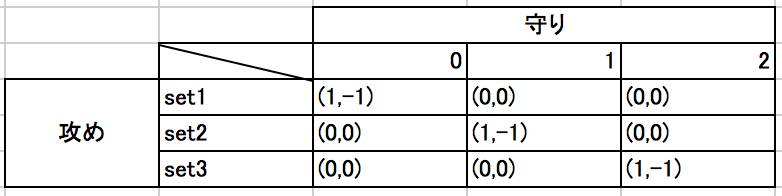
\includegraphics[width=10cm]{pmat.png}
    \caption{利得表}
\end{figure}

これは2人対称ゼロサムゲームとなる。守り手が$\left\{ 0,1,2\right\}$をそれぞれ取る確率を$(q,r,s)$で表記し、攻め手が取るsetに対しての混合戦略、すなわちset1, set2, set3をとる確率を$(x,y,z)$で表記する。この時の混合戦略ナッシュ均衡は以下のようである。
\begin{itembox}[l]{case1 : 完全に合理的な主体を想定したナッシュ均衡}
    \begin{align}
    	\begin{cases}
		(q, r, s) = (\frac{1}{3}, \frac{1}{3}, \frac{1}{3})\\
		(x, y, z) = (\frac{1}{3}, \frac{1}{3}, \frac{1}{3})
	\end{cases}
    \end{align}
\end{itembox}

つまり攻め手も守り手も自身の行動に等しく確率を割り振るのが最適反応を構成している。この時攻め手の本来の行動である$9$個の「宣言」と「指」のペアに対しても等しく$\frac{1}{9}$ずつ確率が振られている。

\section{研究の目的意識}
しかし上記のように全ての戦略に等しく確率を割り振る戦略が実際のプレイでは取られていない可能性が高い。$[a,b]$で宣言$a$ゆびの数$b$の攻め手の行動を表すことにすると、経験的には$[2,1]$のようなある種中途半端な戦略が$[0,0]$や$[4,2]$のような極端な戦略よりも取られやすい傾向があるようように思える。実際、地域によっては利得構造は変えずに$[0,0]$と$[4,2]$に対して特別な名称を与え、他の行動とは別物として扱われているようである。

まず既存の限定合理性のモデル化によって上記の現象が説明できないかを考える。2人完備情報ゲームに適用可能な限定合理生のモデルとして代表的なものには、均衡を扱う概念としてOsborn and Rubinshtein (1998)で提案されたS(k) EquilibriumやMcKelvey and Palfrey (1995)で提案されたquantal response equilibriumがある。しかし、先に挙げたこのゲームの利得表を見ればわかる通りゆびすまは対称なゲームである。このような単純な構造を持つゲームにおいて均衡下で特定の行動が選ばれがちになるような均衡概念は既存のモデル考えにくい。実際、上記のS(k) equilibriumでは均等に行動するのが均衡下での行動であり、QREにおいても通常用いられるoptimization errorの分布を用いると均等に行動するのが均衡として得られてしまう。

そこで、プレイヤーが自身の戦略や相手の戦略について正しい認知を持てていない、つまり限定合理性というよりも根本的にゲームのルールを把握できていないことにナッシュ均衡がプレイされない原因があるのではないかという仮説を立てる。ここでは、「相手の指を一本ずつ別の主体が動かしているものだと見る」と「自身の行動についてどの組み合わせが無差別かを分かっていない」の二つの原因があると想定し、各誤認が発生している時に攻め手がどのような行動をとるかをモデルから導き、データよりそれぞれの誤認の有無を検証する。

また、一つ目にあげた「相手の指を一本ずつ別の主体が動かしているものだと見る」という誤認はそうとわかっても直せないタイプの誤認であるように思える。つまり、ゆびすまをプレイする前に研究者から「相手の指を別々のものとして見る傾向がある」と指摘されても、適切な修正を施して行動できる攻め手は少ないように思える。一方で、二つ目に挙げた「自身の行動についてどの組み合わせが無差別かを分かっていない」については、「自分の宣言数と指の数の差だけが勝敗を消している」というゲームの構造を理解する手助けをするだけで攻め手は行動を適切に修正することができるように思える。このように、認知の歪みには言われて直せるものと言われても直せないものが存在するということを実験を通して明らかにする、

\end{document}





























